\chapter{Widerstandsbestimmung (FT)}\label{s:widerstandsbestimmung}

Das Ziel dieser Arbeit ist es, festzustellen, ob die hybride aktive Str"omungsbeeinflussung von stumpfen K"orpern mittels gepulster Druckluftjets "uber zwei rotierende Coand\^{a}-Walzen mit kleiner Zahnzahl an der K"orperr"uckseite eine nennenswerte Widerstandsreduktion gegen"uber dem Fall ohne Beeinflussung erzielt.

Hierzu muss aus den Versuchsdaten einerseits die jeweiligen Widerstandswerte des K"orpers bestimmt werden. Andererseits ist es erforderlich, abzusch"atzen, ob diese Form der Str"omungsmodifikation unter dem Schlussstrich Energie einsparen kann oder f"ur die Aktuationsmechanismen m"oglicherweise sogar mehr Energie aufgewandt werden muss, als an Einsparung gewonnen werden kann.
Zus"atzlich ist es von Interesse zu bestimmen, wie gro\ss{} der Impuls ist, der durch die Aktuation in die Str"omung eingebracht wird.

Die Gleichungen f"ur diese Zwecke sollen in diesem Kapitel hergeleitet und erl"autert werden.

\section{Bestimmung des Widerstands mittels des Impulssatzes}

Die nachfolgenden Ausf"uhrungen orientieren sich eng an  Hucho \cite{Hucho.2011}.

Der Widerstand eines stumpfen K"orpers innerhalb einer Str"omung macht sich als Impulsverlust derselben stromabw"arts bemerkbar. Der gesuchte Widerstand kann somit bestimmt werden, in dem der Geschwindigkeitsverlauf der Str"omung im Nachlauf betrachtet und mittels des Impulssatzes ausgewertet wird. 

Um den Geschwindigkeitsverlauf zu bestimmen, k"onnen mehrere Methoden angewandt werden, wobei im Rahmen dieser Arbeit die Geschwindigkeiten aus den dynamischen Dr"ucken ermittelt werden.

Der Messrechen im Nachlauf liefert hierzu diverse Dr"ucke - statische und dynamische.

Damit wir unser vereinfachtes mathematisches Modell auf die Versuchsdaten anwenden k"onnen, m"ussen die Dr"ucke der einzelnen Sonden in der Form
\begin{center}	
	\begin{equation}
		\overline{p}=\sum_{i=0}^{n}\frac{p_i}{n}
	\end{equation}
\end{center}
zeitlich gemittelt werden.
Die Summe aller "uber einen Zeitraum genommenen Dr"ucke $p_i$ wird hierbei durch die Anzahl $n$ dieser Dr"ucke innerhalb dieses Zeitraums geteilt.

"Uber den die Definition des dynamischen Drucks $q$ bzw. den Zusammenhang
\begin{center}
	\begin{equation}
		\label{geschwindigkeitsformel}
		u_{1}(y)= \sqrt{\frac{2}{\rho}(p_g - p_{\infty}) } = \sqrt{\frac{2}{\rho} q(y)}
	\end{equation}
\end{center}
l"asst sich wie oben beschrieben der Geschwindigkeitsverlauf aus den gemessenen Dr"ucken bestimmen.

Wobei $u_{1}$ die Str"omungsgeschwindigkeit im Nachlauf in Abh"angigkeit der y-Koordinate und $q$ der gemessene dynamische Druck ist.

Der Widerstand des K"orpers selber l"asst sich nun finden, wenn ein Kontrollvolumen wie in \abb{fig:HuchoKV} um den K"orper gelegt und eine Impulsbilanz aufgestellt wird \cite{Hucho.2011}. Es wird im Folgenden vereinfacht von einer horizontalen, inkompressiblen 2D-Str"omung ausgegangen und der Impulssatz in x-Richtung

\begin{equation}
	\label{eq:impulssatz_allg}
	\rho \int_{(K)} v_x \, \mathrm{d}Q = F_{Kx} + F_{Px} + F_{Sx}
\end{equation}
betrachtet.

Die Dichte der umstr"omenden Luft wird hierbei mit $\rho$ bezeichnet.
Zudem entspricht in \glg{eq:impulssatz_allg} $F_{Kx}$ den angreifenden Volumenkr"aften, $F_{Px}$ der am freien Teil des Volumen angreifenden Oberfl"achenkr"af (Druckkraft) und $F_{Sx}$ der St"utzkraft.

\begin{figure}[h]
	\centering
	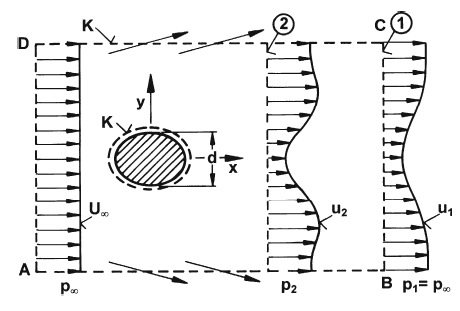
\includegraphics[width=0.5\textwidth]{KontrollvolumenHucho.png}
	\caption{Kontrollvolumen K um einen K"orper mit Geschwindigkeitsverteilungen u(x,y)~\cite{Hucho.2011}}
	\label{fig:HuchoKV}
\end{figure}

Die Volumenkraft $F_{Kx}$ kann dabei zu null gesetzt werden, da die Str"omung in Richtung x horizontal verl"auft und auch abgesehen von der Gewichtskraft keine anderen Volumenkr"afte wirken.

Wenn das Kontrollvolumen, wie es in \abb{fig:HuchoKV} zu sehen ist, weit genug ab vom K"orper gelegt ist, herrscht an den Begrenzungr"andern AD, BC, AB und DC der konstante Druck $p_{\infty}$.
Dies resultiert in einer Druckkraft $F_{Px} = 0$, da sich die Kr"afte an den R"andern aufheben.

Die St"utzkraft kann nun also dem Nettoimpulsfluss gleichgesetzt werden:
\begin{equation}
	\label{eq:nettoimpulsfluss}
	\rho \int_{(K)} \, v_x \, \mathrm{d}Q	= -\rho b \int u_1(u_{\infty} - u_1) \mathrm{d}y = F_{Sx}.	
\end{equation}
Hier ist $b$ die Breite des Modells senkrecht zur Zeichenebene und $U_{\infty}$ die Geschwindigkeit der umgest"orten Anstr"omung.

Die St"utzkraft des festen Teils des Kontrollvolumens - also des Stumpfk"orpers - h"angt mit dem Widerstand in der Form
\begin{equation}
	\label{eq:W=-F_Sx}
	W = - F_{Sx}
\end{equation}
zusammen. 
$W$ ist also gleich der St"utzkraft mit negativem Vorzeichen.

Daraus folgt der Ausdruck f"ur den Widerstand zu
\begin{center}
	\begin{equation}
		\label{eq:widerstand}
		W = \rho b \int u_{1} (u_{\infty}- u_{1}) dy.
	\end{equation}
\end{center}

Der Widerstand l"asst sich dimensionslos und somit vergleichbarer "uber den Widerstandsbeiwert $C_w$ ausdr"ucken. Dieser ist als 
\begin{center}
	\begin{equation}
		\label{eq:def-c_w}
		C_w = \frac{W}{\frac{\rho}{2}}\, U_{\infty}^2 \, bd
	\end{equation}
\end{center}
definiert.

Nach Einsetzen der Gleichung \ref{eq:widerstand} ergibt sich f"ur den Widerstandsbeiwert
\begin{equation}
	\label{eq:Bestimmungsgleichung C_w}
	C_w = \frac{2}{U_{\infty}^2 d} \int u_{1}(U_{\infty} - u_{1}) dy.
\end{equation}
Die Integrationsgrenzen m"ussen an die vertikale Ausdehnung der Sonden am Messrechen im Nachlauf angepasst werden.	

Mit Hilfe dieser Formeln kann dann ein m"ogliche Reduktion des Widerstandsbeiwertes festgestellt werden.

Diese Vorgehensweise ist legitim, wenn an der Messstelle im Nachlauf n"aherungsweise angenommen werden kann, dass der statische Druck wieder $p_\infty$ entspricht und sich die Druckterme im Impulssatz auf  beiden Seiten des Kontrollvolumens gegenseitig aufheben.
Wird die Nachlaufdelle hingegen n"aher am K"orper gemessen, weicht der dort gemessene statische Druck von $p_{\infty}$ ab. Dies  kann nach \textit{B.M. Jones}, wie sie beispielsweise bei \textit{Schlichting} \cite{Schlichting.2001} zu finden ist, durch eine Korrektur ber"ucksichtigt werden.

Hierbei werden die Dr"ucke, die theoretisch an einem Querschnitt $1$ weit genug weg vom K"orper und somit von der statischen Druckabweichung herrschen, auf Dr"ucke zuruckgef"uhrt, die n"aher am K"orper tats"achlich gemessen werden.
Der neue Querschnitt, bei welchem die Messung stattfindet, erh"alt den Index $(2)$.

Der Widerstand in diesem Fall ergibt sich zu

\begin{equation}
	\label{eq:widerstand_korrigiert}
	W = 2b \int \sqrt{p_{t2} - p_2} \left(\sqrt{p_{t\infty} - p_{\infty}} - \sqrt{p_{t2} - p_{\infty}}\right) \mathrm{d} y_2 .
\end{equation}
Wobei $p_{t2}$ und $p_{t\infty}$ dem Totaldruck im Nachlaufquerschnitt bzw. dem Totaldruck der ungest"orten Anstr"omung entspricht.

F"ur den Widerstandsbeiwert erh"alt man

\begin{equation}
	\label{eq:C_w_korrigiert}
	C_w = 2 \int_{(2)} \sqrt{\frac{p_{t2} - p_2}{q_{\infty}}}
	\left(1 - \sqrt{\frac{p_{t2} - p_{\infty}}{q_{\infty}}}\right)  \mathrm{d}\left(\frac{y}{d}\right)).
\end{equation}

\section{Effizienzbetrachtung und Impulskoeffizient}

\subsection{Impulskoeffizient}
Der Impulskoeffizient $C_{\mu}$ wird als Ma\ss{} f"ur die Intensit"at der Ausblasung verwendet \cite{ElSayedM..2018} und ist im Falle von kontinuierlicher Ausblasung als 
\begin{equation}
	\label{eq: Def-momentum-coeff}
	C_{\mu} = \frac{\dot{m}_{jet} \cdot U_{jet}}{\frac{1}{2}\rho^2_{\infty}\, \cdot U_{\infty} \cdot A_{ref}}
\end{equation}
definiert.
Dabei entspricht $\dot{m}_{jet}$ dem Massenstrom, der durch die Spalte ausgeblasen wird. $U_{jet}$ bezeichnet die Geschwindigkeit dieses Ausblasestroms.
$A_{ref}$ wiederum dient als Bezugsfl"ache. Im Falle des getesteten Stumpfk"orpers wird als $A_{ref}$ die projizierte Fl"ache der K"orperh"ohe verwendet. \cite{Bilges.2018}

Die Periodizit"at der Ausblasung kann zus"atzlich im Impulskoeffizient ber"ucksichtigt werden und f"uhrt auf die Form \cite{Chabert.2014}
\begin{equation}
	\label{eq:momentum-coeff-oscill}
	\langle{C_{\mu}}\rangle = \frac{\rho_{jet}\langle{U^2_{jet}}\rangle A_{Spalt}}{\frac{1}{2}\rho_{\infty}U^2_{\infty}A_{ref}}.	
\end{equation}
In \glg{eq:momentum-coeff-oscill} steht der $\langle{}\rangle$-Operator f"ur die jeweiligen zeitlichen Mittelwerte und $A_{Spalt}$ bezeichnet die Fl"ache des Ausblasespalts.

Der Duty-Cycle des Signals der Walzen $\alpha$ kann mit betrachtet werden. Daraus folgt f"ur den Impulskoeffizient mit Ber"ucksichtigung der Periodizit"at die Gleichung
\begin{equation}
	\label{eq:momentum-coeff-oscill-alpha}
	\langle{C_{\mu}}\rangle = \alpha C_{\mu}
\end{equation}	 

%F"ur die Geschwindigkeit $U_{jet}$ l"asst sich auf Grund der kontinuierlichen Spalth"ohen"anderung und der daraus resultierenden Periodizit"at festhalten, dass 


Mittels des Impulskoeffizienten kann die Effektivit"at der Ausblasung beschrieben werden.
Auch f"ur den Vergleich zwischen den untersuchten Walzenpaaren ist die Betrachtung des Impulskoeffizienten ma\ss{}geblich.

\subsection{Leistungskoeffizient und Leistungsrate}
Eine alleinige Betrachtung und ein Vergleich der $C_w$-Werte f"ur den Fall ohne Druckluftzuf"uhrung und rotierende Walzen, sowie den Fall mit aktiver Stro"mungsbeeinflussung ist allerdings nicht ausreichend.

Die durch eine Widerstandsreduktion bedingte Leistungseinsparung im Anwendungsfall k"onnte durchaus durch die extern aufzubringende Leistung f"ur Druckluft und Walzenrotation ausgeglichen oder "ubertroffen werden, sodass letztendlich zus"atzliche Energie aufgebracht und der Zweck der Anwendung verfehlt w"urde.

Ob diese Form der Str"omungsbeeinflussung also eine reale Netto-Leistungseinsparung zur Folge hat, muss folglich durch andere Kennzahlen quantifiziert werden.

Zun"achst verwenden wir f"ur die Effizienzbetrachtung eine Leistungsrate $PR$, die als 

\begin{equation}
	\label{eq:leistungsrate}
	PR = \frac{(W_0 - W)\cdot u_{\infty}}{\frac{1}{2} \dot{m_j} u_j^2 + 2     P_M}
\end{equation}
eingef"uhrt wird.

Der Z"ahler dr"uckt die eingesparte Widerstandsleistung des Falls mit aktiver Str"omungsbeeinflussung im Vergleich mit dem neutralen Fall aus.
Dieser Term quantifiziert somit, in welchem Umfang die Energiedissipation in der Str"omung im zweiten Versuch reduziert wurde.

Der Nenner hingegen repr"asentiert hingegen die Leistung welche dem Modell bzw. der Str"omung von externer Quelle zugef"uhrt werden muss, um den gew"unschten Effekt zu erzielen.

Der erste Summand $\frac{1}{2}\,\dot{m_j} u_j^2$ charakterisiert die kinetische Leistung der Druckluft-Jets, die durch die Spalte ausgeblasen werden. Diese Darstellung vernachl"assigt, dass die  Druckluftbeaufschlagung in den Leitungen Verluste mit sich tr"agt und auch der Kompressor selber keinen optimalen Wirkungsgrad besitzt. Somit handelt es sich bei diesem Term um die idealisierte Jet-Leistung.

Der zweite Summand tr"agt dem Zustand Rechnung, dass die rotierenden Walzen, die verschiedenen Widerst"ande erleiden, von zwei Elektromotoren angetrieben werden m"ussen.
Diese Leistung wird mittels eines Leistungsmessger"ates ermittelt.


Des Weiteren wird als weitere Gr"o\ss{}e noch der Leistungskoeffizient $C_{Power}$ ben"otigt, welcher als
\begin{equation}
	\label{eq:def-powercoefficient}
	C_{Power} = \frac{E_{jet}\dot{m}_{jet} + p_{jet}U_{jet}A_{jet} - (E_p\dot{m}_a + p_p U_p A_p)}{\frac{1}{2}\rho_{\infty}U^2_{\infty} A_{ref}}
\end{equation}

mit
\begin{equation}
	\label{eq:def-energieterm}
	E = c_vT + \frac{U^2}{2}
\end{equation}		
definiert ist.

Gr"o\ss{}en mit Indize $p$ entsprechen dabei den Gr"o\ss{}en innerhalb des Plenums, in dem die Str"omung nicht kontrahiert wird.
Des Weiteren bezeichnet $c_v$ die spezifische W"armekapazit"at von Luft bei konstantem Volumen, $T$ die Temperatur der Luft und $U$ die Geschwindigkeit.

Dieser Koeefiziet dru"ckt das Verh"altinis der aufzubringenden Leistung durch die Aktuation zur in der Antsr"omung vorhandenen Leistung aus.


